\documentclass[11pt, a4paper]{article}
\usepackage[T1]{fontenc}
\usepackage[utf8]{inputenc}
\usepackage[brazil]{babel}
\usepackage{graphicx}  % Uso de figuras.
\usepackage{microtype}  % Melhorias de justificação do texto.
\usepackage{multirow}  % Tabela com várias linhas em uma célula.
\usepackage{lmodern}  % Usa a fonte Latin Modern.
\usepackage{authblk}  % Autor e Afiliação (instituição) do artigo;
\usepackage{bm,array}  % Tabela customizada;
%\usepackage{unifor-enc-cient}  % Modelo UNIFOR - Encontros Científicos 2016
\usepackage{unifor-enc-docen}  % Modelo UNIFOR - Encontro Iniciação à Docência 2016

%------------------------------------------------------------
% Marca d'agua "Rascunho"
%------------------------------------------------------------
\usepackage{draftwatermark}
\SetWatermarkText{Rascunho}
\SetWatermarkScale{1}
\SetWatermarkColor[gray]{0.9}



%------------------------------------------------------------
% BIBLIOGRAFIA
% Substituto do Bibtex
%------------------------------------------------------------
\usepackage[
	backend = biber,
	style = abnt,  % Para usar o sistema alfabético;
%	style = abnt-numeric,  % Para usar o sistema numérico;
%	bftitles,  % Negrito nos títulos;
	giveninits,  % Abrevia primeiros nomes;
	hyperref,  % Criar hyperlinks (se hyperref for usado?);
	backref  % Contar quantas vezes entrada foi citada;
]{biblatex}



% ----------------------------------------------------------
% Define Macro para inserir "palavras-chaves"
% ----------------------------------------------------------
\newcommand{\keywords}[1]{\noindent Palavras-chave: \textit{#1}}



%------------------------------------------------------------
% Arquivo da bibliografia ".bib";
%------------------------------------------------------------
\addbibresource{bibliografia/LabFisica.bib}











%===========================
% Título do Trabalho
%===========================
\title{Lançamento horizontal: um experimento de física básica utilizando Arduino}


%------------------------------------------------------------
% Ordem dos Autores:
% - Primeiro autor: Apresentador do trabalho (com email);
% - Último autor: Orientador (com email).
%------------------------------------------------------------
\author[1]{Raul Fontenele Santana (IC)\thanks{raulfontenele@edu.unifor.br}}
\author[1]{Rodrigo Alves Patrício (PQ)}
\author[1]{Jorge Andre Costa dos Santos (PQ)}
\author[2]{Francisco de Assis Leandro Filho (PQ)}
\author[1]{Roberto Lima da Costa Cisne Júnior (PQ)\thanks{robertolima@unifor.br}}


%------------------------------------------------------------
% Instituições
%------------------------------------------------------------
\affil[1]{Universidade de Fortaleza - UNIFOR}
\affil[2]{Instituto Federal de Educação, Ciência e Tecnologia do Ceará - IFCE}


















%====================================
% INICIO DO DOCUMENTO (de 4 a 6 páginas)
%====================================
\begin{document}

\maketitle



%------------------------------------------------------------
% Palavras Chave: máximo 5, separadas por ponto
%------------------------------------------------------------
\keywords{Laboratório didático. Física. Arduino.}



%===========================
% RESUMO (máximo 250 palavras)
%===========================
\begin{abstract}

\noindent
Um dos problemas enfrentados pelos estudantes de ciências e engenharias está relacionado à dificuldade em compreender alguns fenômenos físicos fundamentais.
O laboratório didático de Física pode ser visto como uma ferramenta que auxilia no aprendizado, assim como um acelerador do mesmo.
Porém, o método clássico usado nas execuções das práticas pode ser algo tedioso sob o ponto de vista tecnológico e social da atualidade.
Na era dos \emph{smartphones}, \emph{ultrabooks}, e internet de alta velocidade, existem inúmeros dispositivos eletrônicos que podem ser usados em procedimentos práticos nto laboratório.
Neste trabalho, utilizamos um experimento de Física já estabelecido nos laboratórios didáticos de Física da UNIFOR, e apresentamos um estudo inicial onde adaptamos a prática sobre lançamento horizontal utilizando a plataforma aberta Arduino.
Os resultados preliminares foram bastante satisfatórios visto que a leitura das medidas utilizando o Arduino foram mais precisas, além do tempo de execução dos procedimento ter sido reduzido. Assim concluímos que a plataforma é de viável de implementação nos laboratórios, porém há necessidade de mais estudos envolvendo práticas relacionadas à outros fenômenos físicos.

\end{abstract}



%==================================
% INTRODUÇÃO
%==================================
\section{Introdução}
%---------------------------------------------------------

A Física é uma disciplina que muitas vezes remete à cálculos e fórmulas matemáticas.
Frequentemente é deixado de lado o teor experimental da mesma, da validade das teorias, dentro do contexto epistemológico.
Porém nos últimos anos vem se dando cada vez mais importância aos laboratórios experimentais, pois estes são apresentados como facilitadores da aprendizagem
\cite{Grandini_2004, Marineli_2006, Souza_2011, RodriguesCunha2014}.
A motivação para aprender também é outro aspecto que deve ser ressaltado no âmbito do laboratório.
Procedimentos arcaicos podem ser uma barreira ao aprendizado, visto o atual momento tecnológico.
Muitos dispositivos de baixo custo estão disponíveis no mercado, os quais desempenham papel importante da automatização de tarefas.
Talvez o exemplo mais evidente seja a plataforma aberta \emph{Arduino}, cuja acessibilidade e facilidade de uso são os pontos chaves deste dispositivo~\cite{OliveiraZanetti2015}.
Não são necessário conhecimentos profundos sobre circuitos para se construir um projeto cheio de elementos eletrônicos que outrora apenas peritos podiam desenvolver.
Fóruns online e uma ampla documentação disponível tornam o aprendizado desta plataforma extremamente viável para qualquer pessoa com acesso à internet.


Segundo \textcite{OliveiraZanetti2015}:
\begin{quote}
``O Arduino é uma plataforma de hardware open source, projetada sobre o microcontrolador Atmel AVR, que pode ser programado através de uma linguagem de programação similar a C/C++, permitindo a elaboração de projetos com um conhecimento mínimo ou mesmo nenhum de eletrônica.
Foi criado com o objetivo de fornecer uma plataforma de fácil prototipação de projetos interativos, unindo software e hardware, características da Computação Física.''
\end{quote}


A utilização de plataformas que envolvem programação computacional por parte do estudante podem causar um impacto positivo na aprendizagem de forma geral.
Os algoritmos computacionais estão intimamente ligados ao desenvolvimento de estruturas do raciocínio lógico, influenciando até no comportamento humano frente à tomada de decisões em problemas do cotidiano~\cite{Wing_2008, Zanetti_2015}.
Além disso, o contato do aluno com o equipamento de modo que o mesmo possa entender seu funcionamento é tanto motivador quanto desmistificador das atividades experimentais \cite{Rosa2003}.

O objetivo deste trabalho é fazer um estudo inicial sobre a viabilidade de construção de um dispositivo de baixo custo, que utilize a plataforma Arduino.
Para isso foi escolhido a prática sobre Lançamento Horizontal, contida no manual do laboratório de Física 1 da UNIFOR.
O dispositivo final deve possuir uma melhor precisão na obtenção de dados quando comparado ao método tradicional usado.




%\textcite{Grandini_2004}, objetivo do laboratório didático na visão dos alunos.

%\textcite{Marineli_2006}, dificuldades nos laboratórios de física;

%\textcite{Souza_2011}, arduino baixo custo, física.

%\textcite{RodriguesCunha2014}, texto de apoio aos professores de física.

%\textcite{OliveiraZanetti2015}, afirma que o Arduino é uma plataforma aberta

%\textcite{Andrades_2013}, periodímetro.





%==================================
% METODOLOGIA
%==================================
\section{Metodologia}
%---------------------------------------------------------


Na Figura~\ref{fig:desenho_lancador} podemos observar a ilustração do lançador horizontal (à esquerda), e o sistema de referência adotado para o estudo (à direita).
Uma esfera de massa $m$ é liberada de um determinado ponto (1 ou 2), e devido a geometria do lançador uma determinada velocidade é atingida na extremidade de lançamento.
Esta velocidade é definida como a velocidade inicial $\vec{v}_o$, pois a partir deste ponto começamos a analisar o movimento, juntamente com o tempo.
Neste trabalho, a esfera sempre é liberada da posição 1, e utilizamos esferas de massas diferentes.
O deslocamento $x$ representa a componente horizontal do movimento, enquanto o $y$ está relacionado com a altura entre o ponto de lançamento e a bancada (posição final).
Três medidas de tempos são realizadas para a obtenção de um tempo médio, o qual é utilizado nos cálculos.
Os fundamentos para o estudo deste tipo de situação, juntamente com todas as equações, não serão analisados visto que já estão bem estabelecidas na literatura básica dos cursos de engenharia~\cite{Resnick2012v1, Moyses2013v1}.



\begin{figure}[!hbt]
\centering
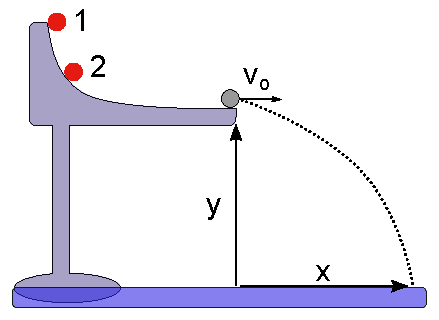
\includegraphics[scale=0.6]{figs/lancamento_suporte.pdf}
%\hspace{15mm}
%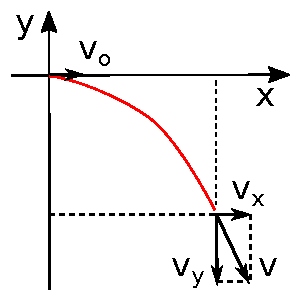
\includegraphics[scale=0.6]{figs/grafico_lancamento.pdf}
\caption{Ilustração do aparato usado no experimento de lançamento horizontal (esquerda), juntamente com o sistema de referência adotado (à direita).}
\label{fig:desenho_lancador}
\end{figure}


Para a realização dos procedimentos utilizamos um suporte universal acoplado com o lançador.
Este dispositivo é o mesmo utilizado nos laboratório didáticos da UNIFOR.
Para a programação do Arduino usamos um laptop convencional com o software Arduino já instalado.
Usamos também vários tipos de sensores conectados ao Arduino. 
A Figura~\ref{fig:aparato_computador} mostra uma fotografia da bancada com os instrumentos utilizados (à esquerda), assim como os componentes Arduino (à direita).
Escolhemos o sensor ultrassônico para a detecção da passagem da esfera na porção final do lançador, e um sensor piezoelétrico para a detecção da chegada da esfera na posição final. Esta escolha dos sensores está relacionada à facilidade de implementação que os mesmo possuem, visto a grande quantidade de manuais e fóruns existentes na \textit{web}.
Já para o procedimento tradicionalmente realizado, além do suporte com o lançador horizontal utilizamos uma régua milimetrada e um cronômetro digital de uso manual.

\begin{figure}[!hbt]
\centering
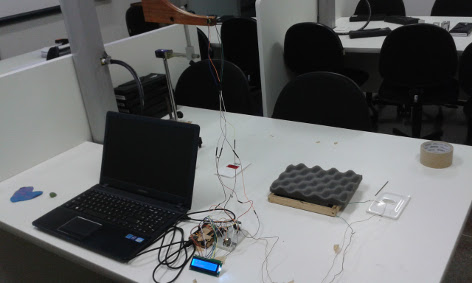
\includegraphics[width=0.45\textwidth]{figs/computador1.jpg}\hspace{5mm}
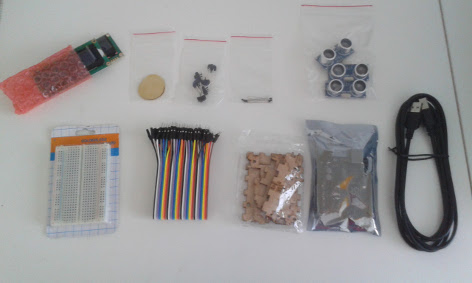
\includegraphics[width=0.45\textwidth]{figs/materiais1.jpg}
\caption{Aparato usado  para verificação de viabilidade de execução de um experimento de teste.}
\label{fig:aparato_computador}
\end{figure}










%==================================
% RESULTADOS E DISCUSSÃO
%==================================
\section{Resultados e Discussão}
%---------------------------------------------------------


O aparato utilizado no experimento sobre lançamento horizontal, está ilustrado na Figura~\ref{fig:aparato_lancamento}.
Os dados para o experimento tradicional, em que um cronômetro digital é manualmente acionado por quem realiza o procedimento, estão de acordo com Tabela~\ref{tab:lancamento_tradicional}.
Já para o caso utilizando Arduino com sensores, estão na Tabela~\ref{tab:lancamento_arduino}.


\begin{figure}[!hbt]
\centering
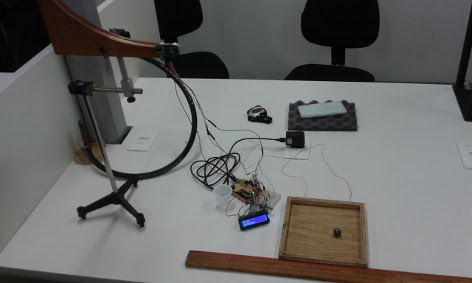
\includegraphics[width=0.3\textwidth]{figs/aparato2.jpg}\hspace{2mm}
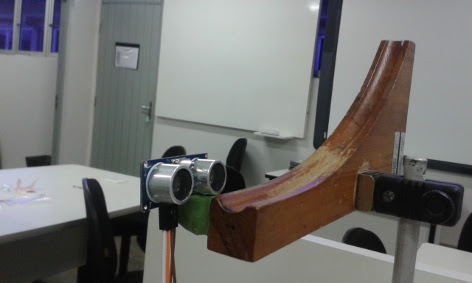
\includegraphics[width=0.3\textwidth]{figs/lancador1.jpg}\hspace{2mm}
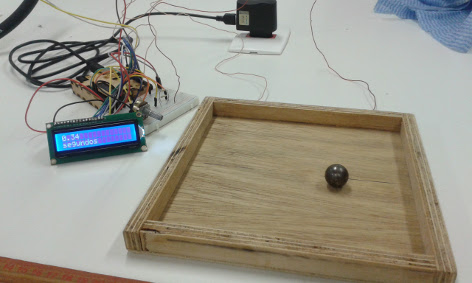
\includegraphics[width=0.3\textwidth]{figs/quadro1.jpg}
\caption{Aparato usado no experimento de lançamento horizontal (à esquerda), juntamente com a saída da medida de tempo pelo sensor, apresentada no visor \textit{LCD} (à direita).}
\label{fig:aparato_lancamento}
\end{figure}




\begin{table}[!hbt]
\centering
\newcolumntype{A}{>{\centering\arraybackslash}p{3.5em}}%Needs 
\newcolumntype{B}{>{\centering\arraybackslash}p{2.5em}}%Needs 
\begin{tabular}{|l|A|A|B|B|B|c|}
\hline 
\multirow{2}{*}{Massas (g)} & \multicolumn{2}{c|}{Deslocamento (cm)} & \multicolumn{3}{c|}{Tempos Medidos (s)} & Tempo Médio\\
\cline{2-7} 
& $y$ & $x$ & $t_1$ & $t_2$ & $t_3$ & $t_m$ \\
\hline 
\hline 
$m_1 = 13,75$ & $50$ & $35$ & $0,34$ & $0,37$ & $0,28$ & $0,33$ \\
\hline 
$m_2 = 23,38$ & $50$ & $33$ & $0,35$ & $0,25$ & $0,31$ & $0,30$ \\
\hline
$m_3 = 48,55$ & $50$ & $30$ & $0,35$ & $0,25$ & $0,25$ & $0,28$ \\
\hline 
\end{tabular}
\caption{Medida dos tempos de queda, em triplicata, para diferentes massas utilizadas no experimento de lançamento horizontal, utilizando o método tradicional.}
\label{tab:lancamento_tradicional}
\end{table}




\begin{table}[!hbt]
\centering
\newcolumntype{A}{>{\centering\arraybackslash}p{3.5em}}%Needs 
\newcolumntype{B}{>{\centering\arraybackslash}p{2.5em}}%Needs 
\begin{tabular}{|l|A|A|B|B|B|c|}
\hline 
\multirow{2}{*}{Massas (g)} & \multicolumn{2}{c|}{Deslocamento (cm)} & \multicolumn{3}{c|}{Tempos Medidos (s)} & Tempo Médio\\
\cline{2-7} 
& $y$ & $x$ & $t_1$ & $t_2$ & $t_3$ & $t_m$ \\
\hline 
\hline 
$m_1 = 13,75$ & $50$ & $35$ & $0,33$ & $0,34$ & $0,32$ & $0,33$ \\
\hline 
$m_2 = 23,38$ & $50$ & $33$ & $0,34$ & $0,34$ & $0,35$ & $0,34$ \\
\hline 
$m_3 = 48,55$ & $50$ & $30$ & $0,34$ & $0,34$ & $0,35$ & $0,34$ \\
\hline 
\end{tabular}
\caption{Medida dos tempos de queda, em triplicata, para diferentes massas utilizadas no experimento de lançamento horizontal, utilizando sensores juntamente com Arduino.}
\label{tab:lancamento_arduino}
\end{table}



Podemos observar que os tempos médios de queda para ambos casos são próximos, porém há uma vantagem quando se usa sensores que detectam a passagem da esfera, pois a flutuação nas medidas dos tempos individuais ($t_1$, $t_2$ e $t_3$) são praticamente ausentes.
Geralmente os resultados utilizando cronômetro acionado manualmente originam erros nos dados~\cite{Andrades_2013}.
O principal fator que origina a imprecisão na leitura do tempo no cronometro manual é a distância $y$ imposta, pois o procedimento é executado em cima da bancada do laboratório.
Uma alternativa seria fazer a esfera cair uma distância maior, por exemplo, até o piso.
Assim um tempo maior seria medido, e haveria uma redução do erro de acionamento manual do cronômetro.
Como estamos tentando realizar os procedimentos na própria bancada, há a necessidade de um dispositivo que faça medidas mais precisas de tempo.


Com o Arduino a precisão das medidas é significativamente melhor, como visto no trabalho realizado por~\textcite{Souza_2011}, o qual aplicou a plataforma em experimentos de física básica (oscilador amortecido, e transferência radiativa de calor).


Durante a realização dos testes de lançamento, alguns outros fatores relacionados ao projeto do aparato vieram à tona.
A colisão entre a esfera e a bancada causa um barulho desagradável.
A posição da esfera no momento em que chega a posição final também é outro parâmetro impreciso. Estes problemas estão sendo trabalhados e serão abordados em trabalhos futuros.




%==================================
% CONCLUSÃO
%==================================
\section{Conclusão}
%---------------------------------------------------------

Neste estudo preliminar, podemos concluir que 
com a utilização da plataforma Arduino em conjunto com alguns sensores, conseguimos obter dados mais precisos para o experimento de lançamento horizontal, quando comparado método tradicional em uso no laboratório de Física da UNIFOR.
A utilização de novos métodos para a realização das práticas nos laboratórios de Física pode ser viável utilizando a plataforma livre Arduino.

Um fator importante para a implementação da plataforma Arduino é seu custo relativamente baixo, assim como dos componentes de circuito.
A precisão das medidas, e a compreensão de como funciona os modernos instrumentos de medida podem ser fatores motivadores do aprendizado, tanto dos conteúdos teóricos da disciplina de Física, quanto da própria Engenharia visto sua essência.




%==================================
% AGRADECIMENTOS
%==================================
\section{Agradecimentos}
%---------------------------------------------------------

Agradecemos à UNIFOR, por ceder os laboratórios didáticos de Física durante algumas tardes, onde pudemos realizar reuniões e montar os experimentos.
Assim como agradecer aos técnicos de laboratório: Carlos Alberto, David Saraiva, Iranildo e Hermesson, pelo suporte técnico, e ao professor Diego Araújo Frota, por algumas discussões sobre o trabalho.



%=====================================
% REFERÊNCIAS (formatação ABNT automática)
%=====================================
\printbibliography




%==== FIM =======================
\end{document}
